%Preamble
\documentclass[newPxFont]{beamer}
\usetheme{sthlm}
%\usecolortheme{sthlmv42}
%-=-=-=-=-=-=-=-=-=-=-=-=-=-=-=-=-=
%        Packages
%-=-=-=-=-=-=-=-=-=-=-=-=-=-=-=-=-=
\usepackage[utf8]{inputenc}
\usepackage{chronology}
\usepackage{hyperref}
\usepackage{amsmath}
\usepackage{amssymb}
\usepackage{booktabs}
%----------------------------------
%Comandos:
\newcommand \imageFrame[2]{
\begingroup
\begin{frame}
  \begin{center}
\includegraphics[width=4in]{#1}\\
\Large #2
    \end{center}
\end{frame}
\endgroup
}

\renewcommand{\event}[3][e]{%
  \pgfmathsetlength\xstop{(#2-\theyearstart)*\unit}%
  \ifx #1e%
    \draw[fill=black,draw=none,opacity=0.5]%
      (\xstop, 0) circle (.2\unit)%
      node[opacity=1,rotate=45,right=.2\unit] {#3};%
  \else%
    \pgfmathsetlength\xstart{(#1-\theyearstart)*\unit}%
    \draw[fill=black,draw=none,opacity=0.5,rounded corners=.1\unit]%
      (\xstart,-.1\unit) rectangle%
      node[opacity=1,rotate=45,right=.2\unit] {#3} (\xstop,.1\unit);%
  \fi}%
%-=-=-=-=-=-=-=-=-=-=-=-=-=-=-=-=-=-=-
%        Beamer options
%-=-=-=-=-=-=-=-=-=-=-=-=-=-=-=-=-=-=-%\setbeameroption{show notes}
%-=-=-=-=-=-=-=-=-=-=-=-=-=-=-=-=-=-=-
%
%	Information
%
%-=-=-=-=-=-=-=-=-=-=-=-=-=-=-=-=-=-=-
\title{Biomedical Engineering Summer School, Wilhelmshaven 2018}
\subtitle{ Instrumentation, Acquisition and Signal Processing for Biosignals}
%\date{\small{\jobname}}
\date{\today}
\author{\texttt{Gerardo Marx Chávez-Campos\\ Mehmet Y\"uksekkaya}}
\institute{\textit{Instituto Tecnológico de Morelia}}


\hypersetup{
pdfauthor = {Marx: gmarx-cc@itmorelia.edu.mx},
pdfsubject = {Fourier series},
pdfkeywords = {orthogonal function, },
pdfmoddate= {D:\pdfdate},
pdfcreator = {Chavez-Campos}
}

\begin{document}
%Title:
\maketitle
%\begin{frame}[plain]
%	\titlepage
%\end{frame}
\begin{frame}{Contest}
\tableofcontents[]
\end{frame}


%=-=-=-=-=-=-=-=-=-=-=-=-=-=-=-=-
\section{Sequence of numbers}
%=-=-=-=-=-=-=-=-=-=-=-=-=-=-=-=-
%=-=-=-=-=-=-=-=-=-=-=-=-=-=-=-=-
\begin{frame}{Sequence of numbers}
\begin{itemize}
  \item Numbers have been used to represent things and count it.
  \item The counting activity allows to know ``How many?''
\end{itemize}

\begin{figure}
  
\includegraphics[width=3in]{history_of_numbers_by_buzzios}
\end{figure}
\end{frame}
%=-=-=-=-=-=-=-=-=-=-=-=-=-=-=-=-
\begin{frame}
\begin{itemize}
  \item However, human beings observe that numbers are in nature in specific sequences\cite{Nova2017}...
\end{itemize}

\begin{figure}
  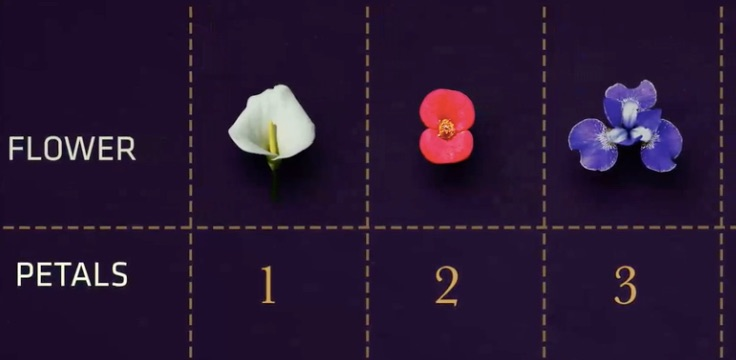
\includegraphics[width=4in]{fibonacci1}
\end{figure}
\end{frame}
%=-=-=-=-=-=-=-=-=-=-=-=-=-=-=-=-
\begin{frame}
\begin{figure}
  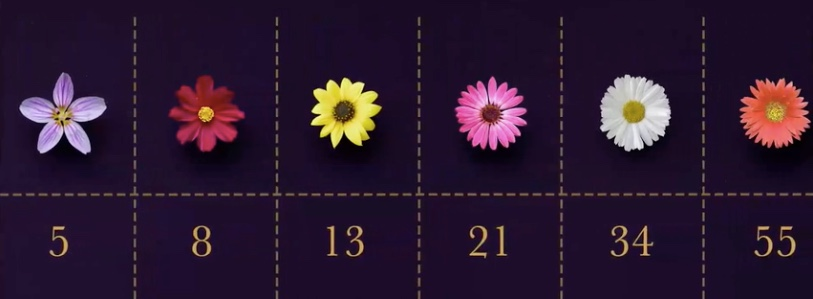
\includegraphics[width=4.3in]{fibonacci2}
\end{figure}
\end{frame}
%=-=-=-=-=-=-=-=-=-=-=-=-=-=-=-=-
\begin{frame}
Let's take a look to this sequence:
\begin{itemize}
  \item 1
  \item 2
  \item 3
  \item 5
  \item 8
  \item 13
  \item 21
  \item 34
  \item 55
  \item ... and so on
\end{itemize}
Can you find some way to relate this numbers?
\end{frame}
%=-=-=-=-=-=-=-=-=-=-=-=-=-=-=-=-
\imageFrame{pine1}{How many spirals can you count?}
%=-=-=-=-=-=-=-=-=-=-=-=-=-=-=-=-
\imageFrame{pine}{The same sequence...}
%%=-=-=-=-=-=-=-=-=-=-=-=-=-=-=-=-
\begin{frame}{The Fibonacci sequence}
The \alert{Fibonacci} sequence is widely found in most nature phenomena. The sequence is easily to create it by the sum of the previos terms:
\begin{eqnarray*}
  u_0=0\\
  u_1=1\\
  u_2=u_0+u_1=0+1=1\\
  u_3=u_1+u_2=1+1=2\\
  u_4=u_2+u_3=2+1=3\\
  %u_5=u_3+u_4=2+3=5\\
  \vdots\\
  u_n=u_{n-1}+u_{n-2}
\end{eqnarray*}
\end{frame}
%=-=-=-=-=-=-=-=-=-=-=-=-=-=-=-=-
\begin{frame}{What is a sequence?}
  \begin{block}{Sequence definition}
    A \textbf{sequence} is a list of things (usually numbers) that are in order:\\
    \begin{equation}
          \underbrace{3}_{\text{1st term}},\underbrace {5}_{\text{2nd term}} ,\underbrace {7}_{\text{3rd term}},\underbrace {9}_{\text{4th term}},\hdots, \underbrace{n}_{\text{nth term}}
    \end{equation}
  \end{block}
  \pause
  A sequence is usually defined by a \alert{Rule}, this is a way or equation to find each term\cite{Math2017}. Thus, in order to be able of determine ($u_n$, $n$th term) the \alert{Rule} is written as a formula, where $n$ is any term.
\end{frame}
%=-=-=-=-=-=-=-=-=-=-=-=-=-=-=-=-
\begin{frame}
    Then, the \alert{Rule} for the sequence $\{ 3,5,7,9,\hdots,\infty\}$ is:
    \begin{table}
      \begin{tabular}{ccc}
     $n$ &\bfseries Term &\bfseries Test rule \\\toprule
     1 & 3 & $2\times 1 +1=3$\\
     2 & 5 & $2\times 2 +1=5$\\
     3 & 7 & $2\times 3 +1=7$\\
     \bottomrule
     \end{tabular}
    \end{table}
\end{frame}
%=-=-=-=-=-=-=-=-=-=-=-=-=-=-=-=-
\begin{frame}{Special sequences}
  \begin{itemize}
    \item <1-> \alert{Arithmetic} sequence has a \alert{constant} value between one term and other e.g. $\{1,4,7,10,13,\hdots\}$, write as an equation: $a_n=a_1+(n-1)d$.
    \item <2-> In the \alert{Geometric} sequence each term is found by multiplying the previous term by a \alert{constant} value: $\{2,4,8,16,32,\hdots,\}$, as an equation:  $a_n=a_1\cdot r^{n-1}$.
    \item <3-> The \alert{Triangular} sequence is generated from dots patterns that form triangles: $\{1,3,6,10,15,21,\}= n(n+1)/2$.
  \end{itemize}
  \visible<4->{\begin{figure}
    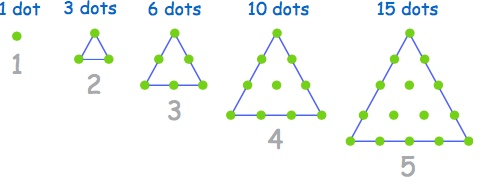
\includegraphics[width=2.5in]{triangular}
  \end{figure}}
\end{frame}
%=-=-=-=-=-=-=-=-=-=-=-=-=-=-=-=-
%Here I am @jade
\imageFrame{exer1}{Matlab time...}
%=-=-=-=-=-=-=-=-=-=-=-=-=-=-=-=-
\section{Series}
\imageFrame{netflix}{No, no this kind of series...}
%=-=-=-=-=-=-=-=-=-=-=-=-=-=-=-=-
\begin{frame}{Finite and infinite series}
  \begin{block}{Finite Series}
    Let ${u_n}$ be a sequence. Then the finite sum (partial sum) order is:\\
    \begin{equation}
        S_k=\sum_{n=1}^{k}=u_1+u_2+u_3+\hdots+u_k
    \end{equation}
  \end{block}
  \pause
  \begin{block}{Infinite Series}
    Let ${u_n}$ be a sequence. Then the Infinite sum order is:\\
    \begin{equation}
        \sum_{n=1}^\infty u_n=u_1+u_2+u_3+\hdots
    \end{equation}
  \end{block}
\end{frame}
%=-=-=-=-=-=-=-=-=-=-=-=-=-=-=-=-
%=-=-=-=-=-=-=-=-=-=-=-=-=-=-=-=-
\begin{frame}{The $n_{th}$ term theorem}
If the partial sums $S_k$ converges to $L$ as $k\longrightarrow \infty$,
  we can say that the infinite series converges and the sum
  tends to $L$ \cite{Math242017}.

\begin{theorem}
If
\begin{equation}
  \lim_{n \to +\infty} U_n=0\label{eq:kthterm}
\end{equation}
the infinity series $\sum_{n=1}^{+\infty} U_n$ is \alert{convergent}
\vspace{0.2in}\\
If
\begin{equation}
  \lim_{n \to +\infty} U_n\neq0
\end{equation}
the infinity series $\sum_{n=1}^{+\infty} U_n$ is \alert{divergent}
\end{theorem}
\end{frame}
%=-==-==-==-==-==-==-==
\imageFrame{L}{A convergent series}
%=-==-==-==-==-==-==-==
%=-==-==-==-==-==-==-==
\imageFrame{exer2}{Let's try it on \alert{Matlab}}
%=-==-==-==-==-==-==-==
\begin{frame}{Does the harmonic series converges?}
Note that the Theorem \eqref{eq:kthterm} not always is true. In other words, it is possible to have a \alert{divergent} series for which $\lim_{n \to +\infty} U_n=0$. An example of such a series is the one known as the harmonic, which is

\pause
\begin{equation}
  \sum_{n=1}^{+\infty} \frac{1}{n}=1+\frac{1}{2}+\frac{1}{3}+\frac{1}{4}+\frac{1}{5}+\frac{1}{6}\cdots+\frac{1}{n}\cdots
\end{equation}
\end{frame}
%=-==-==-==-==-==-==-==
\imageFrame{harmonic}{The harmonic series}
%=-==-==-==-==-==-==-==
%=-==-==-==-==-==-==-==
\imageFrame{exer1}{Improve your code for the harmonic series..}
%=-==-==-==-==-==-==-==
\begin{frame}{More test are required}
Therefore, considering the possibilities in sequences, hence in series, more ways to know if a series  \alert{converges} or \alert{diverges} are needed.
\end{frame}
%=-==-==-==-==-==-==-==
\subsection{The integral test}
\begin{frame}{The integral test}
%The theorem known as the \alert{integral test} makes use of the theory of improper integrals to test an infinite series of positive terms for convergence.
\begin{theorem}
    Let $f$ be a function which is continuous, decreasing, and positive valued for all $x>=1$, then the infinite series
    \begin{equation*}
      \sum_{n=1}^{+\infty} f(n)=f(1)+f(2)+\cdots+f(n)+\cdots
    \end{equation*}
    is \alert{convergent} if the improper integral
    \begin{equation*}
      \int_1^{+\infty} f(x)dx
    \end{equation*}
    exists, and is \alert{divergent} if the improper integral increase without bound.
  \end{theorem}
\end{frame}
%=-=-=-=-=-=-=-=-=-=-=-=-=-=-=-
\subsection{The ratio test}
\begin{frame}
  \begin{theorem}
    Let $\sum a_n$ be an infinite series of nonzero terms and let $L$ to be calculated by \eqref{eq:ratio}
    \begin{equation}
        \lim_{n\to+\infty} \left|\frac{a_{n+1}}{a_n}\right|=L\label{eq:ratio}
      \end{equation}
thus:
\pause
    \begin{itemize}
      \item If $L<1$, the series is absolutely convergent. \pause
      \item If $L>1$, or $L\to\infty$, the series is divergent. \pause
      \item If $L=1$, the series may be absolutely convergent, conditionally convergent, or divergent.
    \end{itemize}
        \end{theorem}
\end{frame}
%=-==-==-==-==-==-==-==-==-==-=


\section{Power series}
\begin{frame}{Power series}
\begin{theorem}
  Let $x$ be a variable. \alert{A power series in $x$} is a series of the form:
  \begin{equation}
    \sum_{n=0}^{\infty} a_n x^n=a_0+a_1 x+a_2 x^2+\cdots+a_n x^n+\cdots
  \end{equation}
  where each $a_n$ is a real number\cite{Swokowski1983}.
\end{theorem}
\end{frame}
%=-==-==-==-==-==-==-==-==-==-=
%=-==-==-==-==-==-==-==-==-==-=
\begin{frame}{Exercise:}
  Find all values of $x$ for which the following power series is absolutely convergent:
  \begin{eqnarray}
    1+\frac{1}{5}x+\frac{2}{5^2}x^2+\cdots+\frac{n}{5^n}x^n+\cdots
  \end{eqnarray}
  \alert{use the ratio test!}
\end{frame}
%=-==-==-==-==-==-==-==-==-==-=
\imageFrame{geometryc}{convergency radius}
%=-==-==-==-==-==-==-==-==-==-=
\subsection{Power series convergency}
\begin{frame}{Power series convergency theorem}
\begin{theorem}
  If $\sum a_n x^n$ is a power series, then precisely one of the following is true
  \begin{itemize}
    \item The series converges only if $x=0$,
    \item The series is absolutely convergent for all $x$,
    \item There is a positive number $r$ such that the series is absolutely convergent if $|x|<r$ and divergent if $|x|>r$
  \end{itemize}
\end{theorem}
\end{frame}
%=-==-==-==-==-==-==-==-==-==-=
\imageFrame{exercise}{Exercise time..}
%=-=-==-=-==-=-==-=-==-=-==-=-==-=-=
\begin{frame}{Power series $(x-c)$}
\begin{theorem}
  Let $c$ be a real number and $x$ a variable. \alert{A power series in} $(x-c)$ is a series of the form
  \begin{equation}
    \sum_{n=0}^{+\infty}a_n (x-c)^n=a_0+a_1(x-c)+a_2(x-c)^2+\cdots+a_n(x-c)^n+\cdots
  \end{equation}
  where each $a_n$ is a real number.
\end{theorem}
\end{frame}
%=-==-==-==-==-==-==-==-==-==-=
\imageFrame{geometryc2}{convergency radius}
%=-==-==-==-==-==-==-==-==-==-=
\subsection{Power series representations of functions}
\begin{frame}{Power series representations of functions}
  A \alert{power series} $\sum a_nx^n$ can be used to define a function of $f(x)$ whose domain is the interval of convergence of the series. Specifically, for each $x$ in this interval we let $f(x)$ equal the sum of the series, that is
  \begin{equation}
    f(x)=a_0+a_1x+a_2x^2+\cdots+a_nx^n+\cdots
  \end{equation}
If a function $f(x)$ is defined in this way we say that $\sum a_nx^n$ is \alert{a power series representative for $f(x)$}.

\alert{This allows us to find values in a new way}. Specifically, if $c$ is the interval of convergence, thus $f(c)$ can be found  or approximated ($\simeq$) be the series.
\end{frame}
%=-==-==-==-==-==-==-==-==-==-=
\subsection{Derivatives and integrals}
\begin{frame}{Derivatives}
  \begin{theorem}
    Suppose a power series $\sum a_nx^n$ has a nonzero radius of convergence $r$ and let the function $f$ be defined by
    \begin{equation}
      f(x)=\sum_{n=0}^{\infty}a_nx^n\label{eq:powerSeries}
    \end{equation}
for every $x$ in the interval of convergence. If $-r<x<r$, then:
    \begin{eqnarray}
      f'(x)=\sum_{n=0}^{\infty}D_x(a_nx^n)=\sum_{n=1}^\infty na_nx^{(n-1)}\label{eq:derivative}\\\nonumber
      =a_1+2a_2x+3a_3x^2+\cdots+na_nx^{(n-1)}+\cdots
    \end{eqnarray}
  \end{theorem}
\end{frame}
%=-==-==-==-==-==-==-==-==-==-=
\begin{frame}{Integral}
\begin{theorem}
\begin{eqnarray}
  \int_0^x f(t)dt=\sum_{n=0}^{\infty}\int_0^x (a_nt^n)dt=\sum_{n=0}^\infty \frac{a_n}{n+1}x^{n+1}\label{eq:integral}\\\nonumber
  =a_0x+\frac{1}{2}a_1x^2+\frac{1}{3}a_2x^3+\cdots+\frac{1}{n+1}a_nx^{n+1}+\cdots
\end{eqnarray}
\end{theorem}
  \begin{alertblock}{to consider}
    as can be shown in Equations \eqref{eq:derivative} and \eqref{eq:integral} the convergency radius remains equal to \eqref{eq:powerSeries}.
  \end{alertblock}
\end{frame}
%=-=-==-=-==-=-==-=-==-=-==-=-==-=-=
\section{Tylor and Maclaurin Series}
\begin{frame}{Tylor and Maclaurin Series}
  Suppose a function $f$ is represented by a power series in $(x-c)$, such that
  \begin{equation}
    f(x)=\sum_{n=0}^{+\infty}a_n (x-c)^n=a_0+a_1(x-c)+a_2(x-c)^2+a_3(x-c)^3+\cdots
  \end{equation}
where the domain of $f$ is an open interval containing $c$.
\end{frame}

\begin{frame}
  \begin{eqnarray}
    f'(x)=\sum_{n=1}^\infty na_n(x-c)^{n-1}\\\nonumber
    =a_1+2a_2(x-c)+3a_3(x-c)^2+4a_4(x-c)^3+\cdots\\
    f''(x)=\sum_{n=2}^\infty n(n-1)a_n(x-c)^{n-2}\\\nonumber
    =2a_2+(3\cdot2)a_3(x-c)+(4\cdot3)a_4(x-c)^2+\cdots\\
    f'''(x)=\sum_{n=3}^\infty n(n-1)(n-2)a_n(x-c)^{n-3}\\\nonumber
    =(3\cdot2)a_3+(4\cdot3\cdot2)a_4(x-c)+\cdots
  \end{eqnarray}
\end{frame}

\begin{frame}
  and, for every positive integer $k$,
  \begin{eqnarray}
    f^{(k)}(x)=\sum_{n=k}^{\infty} n(n-1)\cdots(n-k+1)a_n(x-c)^{n-k}
  \end{eqnarray}
  Moreover, each series obtained by differentiation has the same radius of convergence as the original series. Substituting $c$ for $x$ in each of these series representation, we obtain
  \begin{eqnarray}
    f(c)=a_0\\
    f'(c)=a_1\\
    f''(c)=2a_2\\
    f'''(c)=(3\cdot2)a_3\\
    f^{(n)}(c)=n!a_n \to a_n=\frac{f^{(n)}(c)}{n!}
  \end{eqnarray}
\end{frame}

\begin{frame}{Taylor series}
\begin{theorem}
  If $f$ is a function and
  \begin{equation}
    f(x)=\sum_{n=0}^\infty a_n(x-c)^n
  \end{equation}
  for all $x$ in an open interval containing $c$, then
  \begin{equation}
    f(x)=f(c)+f'(c)(x-c)+\frac{f''(c)}{2!}(x-c)^2+\cdots+\frac{f^{(n)}(c)}{n!}(x-c)^n
  \end{equation}
\end{theorem}
\end{frame}

\begin{frame}{Maclaurin}
  \begin{Corollary}
    If $f$ is a function and $f(x)=\sum a_nx^n$ for all $x$ in an open interval $(-r,r)$, then
    \begin{equation}
    f(x)=f(0)+f'(0)x+\frac{f''(0)}{2!}x^2+\cdots+\frac{f^{(n)}(0)}{n!}x^n+\cdots
    \end{equation}
  \end{Corollary}
\end{frame}
%=-==-==-==-==-==-==-==-==-==-=
\imageFrame{homer_at_work}{Come on guys, you almost have done...}
%--------------------
\begin{frame}{References}
	\begin{thebibliography}{10}
	\beamertemplatebookbibitems
  \bibitem{Nova2017}
  [1] Nova foundation for Science
  \newblock Pi \& the Fibonacci sequence
	\bibitem{Zill2009}
  [2] Deniss G. Zill and Michael R. Cullen
	\newblock Differential Equations with Boundary-Valuer Problems
	\bibitem{Math2017}
    [3] Math is Fun
	\newblock www.mathisfun.com

	\bibitem{Math242017}
    [4] Everything you need to master Calculus and Differential Equations
	\newblock www.math24.com

	\beamertemplatebookbibitems
	\bibitem{Swokowski1983}
	[5] Earl W. Swokowski
	\newblock Calculus with analytic geometry
	\newblock Prindle, Weber \& Schmidt, 1979

  \end{thebibliography}
\end{frame}
\end{document}
